\documentclass[empirical, authordate, issue]{jote-new-article}
\addbibresource{bibliography.bib}



\begin{filecontents}{bibliography.bib}
@article{Clifford2014,
  author = {Clifford, S. and Jerit, J.},
  date = {2014},
  title = {Is There a Cost to Convenience? An Experimental Comparison of Data Quality in Laboratory and Online Studies},
  volume = {1},
  pages = {120–131},
  url = {https://doi.org/10.1017/xps.2014.5},
  doi = {10.1017/xps.2014.5},
  journal = {Journal of Experimental Political Science},
  number = {2}
}

    @thesis{Bartlett2020,
    author = {Bartlett, J.E.},
    date = {2020},
    title = {Daily and Non-daily Smokers: A Profile of Drive and Cognitive Control Mechanisms},
    url = {https://thesiscommons.org/h9gpe/},
    school = {Coventry University},
    type = {PhD}
  }

@article{AnwylIrvine2019,
  author = {Anwyl-Irvine, A. and Massonnié, J. and Flitton, A. and Kirkham, N. and Evershed, J.},
  date = {2019},
  title = {Gorilla in our Midst: An online behavioral experiment builder},
  volume = {52},
  pages = {388–407},
  url = {https://doi.org/10.1101/438242},
  doi = {10.1101/438242},
  journal = {Behavior Research Methods}
}

  @article{Shiffman2009,
    title       = {Light and intermittent smokers: Background and perspective},
    author      = {Shiffman, S.},
    number      = {2},
    volume      = {11},
    doi         = {10.1093/ntr/ntn020},
    year        = {2009},
    pages       = {122--125},
    journal     = {Nicotine \& Tobacco Research}
}
@article{Levy2009,
  author = {Levy, D. E. and Biener, L. and Rigotti, N. A.},
  date = {2009},
  title = {The natural history of light smokers: A population-based cohort study},
  volume = {11},
  pages = {156-163},
  url = {https://doi.org/10.1093/ntr/ntp011},
  doi = {10.1093/ntr/ntp011},
  journal = {Nicotine \& Tobacco Research},
  number = {2}
}

@article{Leys2013,
    title       = {Detecting outliers: Do not use standard deviation around the mean, use absolute deviation around the median},
    author      = {Leys, C. and Ley, C. and Klein, O. and Bernard, P. and Licata, L.},
    number      = {4},
    volume      = {49},
    url         = {https://doi.org/10.1016/j.jesp.2013.03.013},
    doi         = {10.1016/j.jesp.2013.03.013},
    year        = {2013},
    pages       = {764--766},
    journal     = {Journal of Experimental Social Psychology}
}


@article{StHelen2019,
  author = {St.Helen, G. and Benowitz, N.L. and Ahluwalia, J.S. and Tyndale, R.F. and Addo, N. and Gregorich, S.E. and Pérez-Stable, E.J. and Cox, L.S.},
  date = {2019},
  title = {Black Light Smokers: How Nicotine Intake and Carcinogen Exposure Differ Across Various Biobehavioral Factors},
  volume = {111},
  pages = {509–520},
  url = {https://doi.org/10.1016/j.jnma.2019.04.004},
  doi = {10.1016/j.jnma.2019.04.004},
  journal = {Journal of the National Medical Association},
  number = {5}
}


@article{Shiffman2012,
    title       = {Smoking motives of daily and non-daily smokers: A profile analysis},
    author      = {Shiffman, S. and Dunbar, M.S. and Scholl, S.M. and Tindle, H.A.},
    number      = {3},
    volume      = {126},
    doi         = {10.1016/j.drugalcdep.2012.05.037},
    year        = {2012},
    pages       = {362--368},
    journal     = {Drug and Alcohol Dependence}
}

@article{Shiffman2012a,
  author = {Shiffman, S. and Tindle, H. and Li, X. and Scholl, S. and Dunbar, M. and Mitchell-Miland, C.},
  date = {2012},
  title = {Characteristics and smoking patterns of intermittent smokers},
  volume = {20},
  pages = {264–277},
  url = {https://doi.org/10.1037/a0027546},
  doi = {10.1037/a0027546},
  journal = {Experimental and Clinical Psychopharmacology},
  number = {4}
}




@article{Bogdanovica2011,
    title       = {Smoking prevalence in the European Union: A comparison of national and transnational prevalence survey methods and results},
    author      = {Bogdanovica, I. and Godfrey, F. and McNeill, A. and Britton, J.},
    number      = {1},
    volume      = {20},
    doi         = {10.1136/tc.2010.036103},
    year        = {2011},
    pages       = {1--9},
    journal     = {Tobacco Control}
}


@article{Kotz2012,
    title       = {Very low rate and light smokers: Smoking patterns and cessation-related behaviour in England, 2006-11: Very low rate and light smokers},
    author      = {Kotz, D. and Fidler, J. and West, R.},
    number      = {5},
    volume      = {107},
    doi         = {10.1111/j.1360-0443.2011.03739.x},
    year        = {2012},
    pages       = {995--1002},
    journal     = {Addiction}
}


@article{Tindle2011,
    title       = {Smoking Cessation Behavior Among Intermittent Smokers Versus Daily Smokers},
    author      = {Tindle, H.A. and Shiffman, S.},
    number      = {7},
    volume      = {101},
    doi         = {10.2105/AJPH.2011.300186},
    year        = {2011},
    pages       = {1-- 3},
    journal     = {American Journal of Public Health}
}


@article{Fagan2009,
    title       = {Light and intermittent smoking: The road less traveled},
    author      = {Fagan, P. and Rigotti, N.A.},
    number      = {2},
    volume      = {11},
    doi         = {10.1093/ntr/ntn015},
    year        = {2009},
    pages       = {107--110},
    journal     = {Nicotine \& Tobacco Research}
}


@article{Tong2006,
    title       = {Nondaily Smokers Should Be Asked and Advised to Quit},
    author      = {Tong, E.K. and Ong, M.K. and Vittinghoff, E. and Pérez-Stable, E.J.},
    number      = {1},
    volume      = {30},
    doi         = {10.1016/j.amepre.2005.08.048},
    year        = {2006},
    pages       = {23--30},
    journal     = {American Journal of Preventive Medicine}
}


@article{Shiffman2014,
    title       = {Smoking Patterns and Stimulus Control in Intermittent and Daily Smokers},
    author      = {Shiffman, S. and Dunbar, M.S. and Li, X. and Scholl, S.M. and Tindle, H.A. and Anderson, S.J. and Ferguson, S.G.},
    number      = {3},
    volume      = {9},
    doi         = {10.1371/journal.pone.0089911},
    year        = {2014},
    pages       = {1--14},
    journal     = {PLoS ONE}
}


@article{Field2008,
    title       = {Attentional bias in addictive behaviors: A review of its development, causes, and consequences},
    author      = {Field, M. and Cox, W.M.},
    number      = {1-2},
    volume      = {97},
    doi         = {10.1016/j.drugalcdep.2008.03.030},
    year        = {2008},
    pages       = {1--20},
    journal     = {Drug and Alcohol Dependence}
}


@article{Field2009,
    title       = {A meta-analytic investigation of the relationship between attentional bias and subjective craving in substance abuse},
    author      = {Field, M. and Munafò, M.R. and Franken, I.H.A.},
    number      = {4},
    volume      = {135},
    doi         = {10.1037/a0015843},
    year        = {2009},
    pages       = {589--607},
    journal     = {Psychological Bulletin}
}


@article{Field2016,
    title       = {The role of attentional bias in obesity and addiction},
    author      = {Field, M. and Werthmann, J. and Franken, I. and Hofmann, W. and Hogarth, L. and Roefs, A.},
    number      = {8},
    volume      = {35},
    doi         = {10.1037/hea0000405},
    year        = {2016},
    pages       = {767--780},
    journal     = {Health Psychology}
}


@article{Baschnagel2013,
    title       = {Using mobile eye-tracking to assess attention to smoking cues in a naturalized environment},
    author      = {Baschnagel, J.S.},
    number      = {12},
    volume      = {38},
    doi         = {10.1016/j.addbeh.2013.08.005},
    year        = {2013},
    pages       = {2837--2840},
    journal     = {Addictive Behaviors}
}


@article{Ehrman2002,
    title       = {Comparing attentional bias to smoking cues in current smokers, former smokers, and non-smokers using a dot-probe task},
    author      = {Ehrman, R.N. and Robbins, S.J. and Bromwell, M.A. and Lankford, M.E. and Monterosso, J.R. and O'Brien, C.P.},
    number      = {2},
    volume      = {67},
    doi         = {10.1016/S0376-8716(02)00065-0},
    year        = {2002},
    pages       = {185--191},
    journal     = {Drug and Alcohol Dependence}
}


@article{Kang2012,
    title       = {Individual differences in smoking-related cue reactivity in smokers: An eye-tracking and fMRI study},
    author      = {Kang, O.-S. and Chang, D.-S. and Jahng, G.-H. and Kim, S.-Y. and Kim, H. and Kim, J.-W. and Chung, S.-Y. and Yang, S.-I. and Park, H.-J. and Lee, H. and Chae, Y.},
    number      = {2},
    volume      = {38},
    doi         = {10.1016/j.pnpbp.2012.04.013},
    year        = {2012},
    pages       = {285--293},
    journal     = {Progress in Neuro-Psychopharmacology and Biological Psychiatry}
}


@article{Mogg2003,
    title       = {Eye movements to smoking-related pictures in smokers: Relationship between attentional biases and implicit and explicit measures of stimulus valence},
    author      = {Mogg, K. and Bradley, B.P. and Field, M. and Houwer, J.},
    number      = {6},
    volume      = {98},
    doi         = {10.1046/j.1360-0443.2003.00392.x},
    year        = {2003},
    pages       = {825--836},
    journal     = {Addiction}
}


@article{Bradley2003,
    title       = {Attentional bias in drug dependence: Vigilance for cigarette-related cues in smokers},
    author      = {Bradley, B.P. and Mogg, K. and Wright, T. and Field, M.},
    number      = {1},
    volume      = {17},
    doi         = {10.1037/0893-164X.17.1.66},
    year        = {2003},
    pages       = {66--72},
    journal     = {Psychology of Addictive Behaviors}
}


@article{Hogarth2003,
    title       = {Attentional orienting towards smoking-related stimuli},
    author      = {Hogarth, L.C. and Mogg, K. and Bradley, B.P. and Duka, T. and Dickinson, A.},
    number      = {2},
    volume      = {14},
    doi         = {10.1097/00008877-200303000-00007},
    year        = {2003},
    pages       = {153--160},
    journal     = {Behavioural Pharmacology}
}


@article{Mogg2005,
    title       = {Attentional and approach biases for smoking cues in smokers: An investigation of competing theoretical views of addiction},
    author      = {Mogg, K. and Field, M. and Bradley, B.P.},
    number      = {2},
    volume      = {180},
    doi         = {10.1007/s00213-005-2158-x},
    year        = {2005},
    pages       = {333--341},
    journal     = {Psychopharmacology}
}


@article{Chanon2010,
    title       = {Attentional bias toward cigarette cues in active smokers},
    author      = {Chanon, V.W. and Sours, C.R. and Boettiger, C.A.},
    number      = {3},
    volume      = {212},
    doi         = {10.1007/s00213-010-1953-1},
    year        = {2010},
    pages       = {309--320},
    journal     = {Psychopharmacology}
}


@article{Vollstädt-Klein2011,
    title       = {Attention Shift towards Smoking Cues Relates to Severity of Dependence, Smoking Behavior and Breath Carbon Monoxide},
    author      = {Vollstädt-Klein, S. and Loeber, S. and Winter, S. and Leménager, T. and Goltz, C.von der and Dinter, C. and Koopmann, A. and Wied, C. and Winterer, G. and Kiefer, F.},
    number      = {4},
    volume      = {17},
    doi         = {10.1159/000327775},
    year        = {2011},
    pages       = {217--224},
    journal     = {European Addiction Research}
}


@article{Zack2001,
    title       = {Effects of abstinence and smoking on information processing in adolescent smokers},
    author      = {Zack, M. and Belsito, L. and Scher, R. and Eissenberg, T. and Corrigall, W.A.},
    number      = {2},
    volume      = {153},
    doi         = {10.1007/s002130000552},
    year        = {2001},
    pages       = {249--257},
    journal     = {Psychopharmacology}
}


@article{Parsons2019,
    title       = {Psychological Science Needs a Standard Practice of Reporting the Reliability of Cognitive-Behavioral Measurements},
    author      = {Parsons, S. and Kruijt, A.-W. and Fox, E.},
    number      = {4},
    volume      = {2},
    doi         = {10.1177/2515245919879695},
    year        = {2019},
    pages       = {378--395},
    journal     = {Advances in Methods and Practices in Psychological Science}
}


@article{Pennington2021,
    title       = {Raising the bar: Improving methodological rigour in cognitive alcohol research},
    author      = {Pennington, C.R. and Jones, A. and Bartlett, J.E. and Copeland, A. and Shaw, D.J.},
    number      = {11},
    volume      = {116},
    doi         = {10.1111/add.15563},
    year        = {2021},
    pages       = {3243--3251},
    journal     = {Addiction}
}


@article{Hedge2018,
    title       = {The reliability paradox: Why robust cognitive tasks do not produce reliable individual differences},
    author      = {Hedge, C. and Powell, G. and Sumner, P.},
    number      = {3},
    volume      = {50},
    doi         = {10.3758/s13428-017-0935-1},
    year        = {2018},
    pages       = {1166--1186},
    journal     = {Behavior Research Methods}
}


@article{Ataya2012,
    title       = {Internal reliability of measures of substance-related cognitive bias},
    author      = {Ataya, A.F. and Adams, S. and Mullings, E. and Cooper, R.M. and Attwood, A.S. and Munafò, M.R.},
    number      = {1},
    volume      = {121},
    doi         = {10.1016/j.drugalcdep.2011.08.023},
    year        = {2012},
    pages       = {148--151},
    journal     = {Drug and Alcohol Dependence}
}


@article{Schmukle2005,
    title       = {Unreliability of the dot probe task},
    author      = {Schmukle, S.C.},
    number      = {7},
    volume      = {19},
    doi         = {10.1002/per.554},
    year        = {2005},
    pages       = {595--605},
    journal     = {European Journal of Personality}
}


@article{Waechter2014,
    title       = {Measuring Attentional Bias to Threat: Reliability of Dot Probe and Eye Movement Indices},
    author      = {Waechter, S. and Nelson, A.L. and Wright, C. and Hyatt, A. and Oakman, J.},
    number      = {3},
    volume      = {38},
    doi         = {10.1007/s10608-013-9588-2},
    year        = {2014},
    pages       = {313--333},
    journal     = {Cognitive Therapy and Research}
}


@article{Fagerström2012,
    title       = {Determinants of Tobacco Use and Renaming the FTND to the Fagerström Test for Cigarette Dependence},
    author      = {Fagerström, K.},
    number      = {1},
    volume      = {14},
    doi         = {10.1093/ntr/ntr137},
    year        = {2012},
    pages       = {75--78},
    journal     = {Nicotine \& Tobacco Research}
}


@article{Heatherton1991,
    title       = {The Fagerström Test for Nicotine Dependence: A revision of the Fagerstrom Tolerance Questionnaire},
    author      = {Heatherton, T.F. and Kozlowski, L.T. and Frecker, R.C. and Fagerström, K.-O.},
    number      = {9},
    volume      = {86},
    doi         = {10.1111/j.1360-0443.1991.tb01879.x},
    year        = {1991},
    pages       = {1119--1127},
    journal     = {British Journal of Addiction}
}


@book{Lang2008,
    title       = {International affective picture system (IAPS): Affective ratings of pictures and instruction manual},
    author      = {Lang, P.J. and Bradley, M.M. and Cuthbert, B.N.},
    publisher   = {University of Florida},
    place       = {Gainesville},
    year        = {2008},
    series     = {Technical Report A-8}
}



@article{Allen2019,
    title       = {Raincloud plots: A multi-platform tool for robust data visualization},
    author      = {Allen, M. and Poggiali, D. and Whitaker, K. and Marshall, T.R. and Kievit, R.A.},
    volume      = {4},
    doi         = {10.12688/wellcomeopenres.15191.1},
    year        = {2019},
    pages       = {63},
    journal     = {Wellcome Open Research}
}


@article{Salemink2007,
    title       = {Selective attention and threat: Quick orienting versus slow disengagement and two versions of the dot probe task},
    author      = {Salemink, E. and Hout, M.A.van den and Kindt, M.},
    number      = {3},
    volume      = {45},
    doi         = {10.1016/j.brat.2006.04.004},
    year        = {2007},
    pages       = {607--615},
    journal     = {Behaviour Research and Therapy}
}


@article{Lakens2018,
    title       = {Equivalence Testing for Psychological Research: A Tutorial},
    author      = {Lakens, D. and Scheel, A.M. and Isager, P.M.},
    number      = {2},
    volume      = {1},
    doi         = {10.1177/2515245918770963},
    year        = {2018},
    pages       = {259--269},
    journal     = {Advances in Methods and Practices in Psychological Science}
}


@article{Simonsohn2015,
    title       = {Small Telescopes: Detectability and the Evaluation of Replication Results},
    author      = {Simonsohn, U.},
    number      = {5},
    volume      = {26},
    doi         = {10.1177/0956797614567341},
    year        = {2015},
    pages       = {559--569},
    journal     = {Psychological Science}
}


@article{Grice2020,
    title       = {Persons as Effect Sizes},
    author      = {Grice, J.W. and Medellin, E. and Jones, I. and Horvath, S. and McDaniel, H. and O'lansen, C. and Baker, M.},
    number      = {4},
    volume      = {3},
    doi         = {10.1177/2515245920922982},
    year        = {2020},
    pages       = {443--455},
    journal     = {Advances in Methods and Practices in Psychological Science}
}


@article{Parsons2020,
    title       = {Splithalf; robust estimates of split half reliability},
    author      = {Parsons, S.},
    doi         = {10.6084/m9.figshare.5559175.v5},
    year        = {2020}
}


@article{Schaefer2019,
  author = {Schäfer, T. and Schwarz, M.A.},
  date = {2019},
  title = {The Meaningfulness of Effect Sizes in Psychological Research: Differences Between Sub-Disciplines and the Impact of Potential Biases},
  volume = {10},
  pages = {1–13},
  url = {https://doi.org/10.3389/fpsyg.2019.00813},
  doi = {10.3389/fpsyg.2019.00813},
  journal = {Frontiers in Psychology}
}


@article{Begh2016,
    title       = {Association between smoking-related attentional bias and craving measured in the clinic and in the natural environment},
    author      = {Begh, R. and Smith, M. and Ferguson, S.G. and Shiffman, S. and Munafò, M.R. and Aveyard, P.},
    number      = {8},
    volume      = {30},
    doi         = {10.1037/adb0000231},
    year        = {2016},
    pages       = {868--875},
    journal     = {Psychology of Addictive Behaviors}
}


@article{Price2015,
    title       = {Empirical Recommendations for Improving the Stability of the Dot-Probe Task in Clinical Research},
    author      = {Price, R.B. and Kuckertz, J.M. and Siegle, G.J. and Ladouceur, C.D. and Silk, J.S. and Ryan, N.D. and Dahl, R.E. and Amir, N.},
    number      = {2},
    volume      = {27},
    doi         = {10.1037/pas0000036},
    year        = {2015},
    pages       = {365--376},
    journal     = {Psychological Assessment}
}


@article{Soleymani2020,
    title       = {Free-viewing multi-stimulus eye tracking task to index attention bias for alcohol versus soda cues: Satisfactory reliability and criterion validity},
    author      = {Soleymani, A. and Ivanov, Y. and Mathot, S. and Jong, P.J.de},
    volume      = {100},
    doi         = {10.1016/j.addbeh.2019.106117},
    year        = {2020},
    pages       = {106117},
    journal     = {Addictive Behaviors}
}


@article{Wray2016,
    title       = {A Comparative Evaluation of Self-Report and Biological Measures of Cigarette Use in Non-Daily Smokers},
    author      = {Wray, J.M. and Gass, J.C. and Miller, E.I. and Wilkins, D.G. and Rollins, D.E. and Tiffany, S.T.},
    number      = {9},
    volume      = {28},
    doi         = {10.1037/pas0000227},
    year        = {2016},
    pages       = {1043--1050},
    journal     = {Psychological Assessment}
}


@article{Ramo2011,
    title       = {Reliability and validity of self-reported smoking in an anonymous online survey with young adults},
    author      = {Ramo, D.E. and Hall, S.M. and Prochaska, J.J.},
    number      = {6},
    volume      = {30},
    doi         = {10.1037/a0023443},
    year        = {2011},
    pages       = {693--701},
    journal     = {Health Psychology}
}

@misc{RCoreTeam2020,
    title       = {R: A language and environment for statistical computing. R Foundation for Statistical Computing},
    author      = {{R Core Team}},
    url         = {https://www.R-project.org/},
    year        = {2020}
}


@misc{Singmann2020,
    title       = {Afex: Analysis of factorial experiments},
    author      = {Singmann, H. and Bolker, B. and Westfall, J. and Aust, F. and Ben-Shachar, M.S.},
    url         = {https://CRAN.R-project.org/package=afex},
    year        = {2020}
}


@misc{Wilke2019,
    title       = {Cowplot: Streamlined plot theme and plot annotations for 'ggplot2'},
    author      = {Wilke, C.O.},
    url         = {https://CRAN.R-project.org/package=cowplot},
    year        = {2019}
}


@misc{Wickham2020,
    title       = {Tidyr: Tidy messy data},
    author      = {Wickham, H. and Henry, L.},
    url         = {https://CRAN.R-project.org/package=tidyr},
    year        = {2020}
}


@book{Wickham2016,
    title       = {ggplot2: Elegant graphics for data analysis},
    author      = {Wickham, H.},
    url         = {https://ggplot2.tidyverse.org},
    publisher   = {Springer-Verlag New York},
    year        = {2016}
}


@misc{Firke2019,
    title       = {Janitor: Simple tools for examining and cleaning dirty data},
    author      = {Firke, S.},
    url         = {https://CRAN.R-project.org/package=janitor},
    year        = {2019}
}


@manual{Aust2022,
    title = {{papaja}: {Prepare} reproducible {APA} journal articles
      with {R Markdown}},
    author = {Frederik Aust and Marius Barth},
    year = {2022},
    note = {R package version 0.1.1},
    url = {https://github.com/crsh/papaja},
  }


@book{Revelle2019,
    title       = {Psych: Procedures for psychological, psychometric, and personality research},
    author      = {Revelle, W.},
    url         = {https://CRAN.R-project.org/package=psych},
    publisher   = {Northwestern University},
    year        = {2019}
}


@misc{Champely2020,
    title       = {Pwr: Basic functions for power analysis},
    author      = {Champely, S.},
    url         = {https://CRAN.R-project.org/package=pwr},
    year        = {2020}
}


@misc{Wickham2018,
    title       = {Readr: Read rectangular text data},
    author      = {Wickham, H. and Hester, J. and Francois, R.},
    url         = {https://CRAN.R-project.org/package=readr},
    year        = {2018}
}


@misc{Chang2020,
    title       = {Shiny: Web application framework for r},
    author      = {Chang, W. and Cheng, J. and Allaire, J. and Xie, Y. and McPherson, J.},
    url         = {https://CRAN.R-project.org/package=shiny},
    year        = {2020}
}


@misc{Wickham2019,
    title       = {Stringr: Simple, consistent wrappers for common string operations},
    author      = {Wickham, H.},
    url         = {https://CRAN.R-project.org/package=stringr},
    year        = {2019}
}


@misc{Müller2020,
    title       = {Tibble: Simple data frames},
    author      = {Müller, K. and Wickham, H.},
    url         = {https://CRAN.R-project.org/package=tibble},
    year        = {2020}
}


@misc{Barth2022,
    title       = {tinylabels: Lightweight variable labels},
    author      = {Barth, M.},
    url         = {https://cran.r-project.org/package=tinylabels},
    year        = {2022}
}


@misc{Lakens2017,
    title       = {Equivalence tests: A practical primer for t-tests, correlations, and meta-analyses},
    author      = {Lakens, D.},
    volume      = {1},
    url         = {https://doi.org/10.1177/1948550617697177},
    doi         = {10.1177/1948550617697177},
    year        = {2017},
    pages       = {1--8},
    journal     = {Social Psychological and Personality Science}
}


\end{filecontents}
\jotetitle{No Meaningful Difference in \mbox{Attentional} Bias Between Daily and Non-Daily Smokers}
\keywordsabstract{attentional bias, daily smokers, non-daily smokers, visual probe task, equivalence testing}
\abstracttext{Both daily and non-daily smokers find it difficult to quit smoking long-term. One factor associated with addictive behavior is attentional bias, but previous research in daily and non-daily smokers found inconsistent results and did not report the reliability of their cognitive tasks. Using an online sample, we compared daily (\emph{n} = 106) and non-daily (\emph{n} = 60) smokers in their attentional bias towards smoking pictures. Participants completed a visual probe task with two picture presentation times: 200ms and 500ms. In confirmatory analyses, there were no significant effects of interest, and in exploratory analyses, equivalence testing showed the effects were statistically equivalent to zero. The reliability of the visual probe task was poor, meaning it should not be used for repeated testing or investigating individual differences. The results can be interpreted in line with contemporary theories of attentional bias where there are unlikely to be stable trait-like differences between smoking groups. Future research in attentional bias should focus on state-level differences using more reliable measures than the visual probe task.}
\runningauthor{Bartlett et al.}
\jname{Journal of Trial \& Error}
\jyear{2022}
% \funding{\undefined}
\paperdoi{10.36850/e11}
\paperreceived{December 13, 2021}
\author[1]{James Bartlett\orcid{https://orcid.org/0000-0002-4191-5245}}
\authortwo{James Bartlett}
\affil[1]{School of Psychology and Neuroscience, University of Glasgow}
\corremail{\href{mailto:james.bartlett@glasgow.ac.uk}{james.bartlett@glasgow.ac.uk}}
\corraddress{School of Psychology and Neuroscience, University of Glasgow}
\author[2]{Rebecca Jenks\orcid{https://orcid.org/0000-0001-6479-539X}}
\authorthree{Rebecca Jenks}
\affil[2]{School of Psychological, Social and Behavioural Sciences, Coventry University}
\author[3]{Nigel Wilson}
\authorfour{Nigel Wilson}
\affil[3]{School of Psychology and Sociology, Arden University}
\paperaccepted{November 15, 2022}
\paperpublished{December 13, 2022}
\paperpublisheddate{2022-12-13}
\jwebsite{https://journal.trialanderror.org}

\begin{document}

\begin{frontmatter}
  \maketitle

  \begin{abstract}
    \printabstracttext
  \end{abstract}
\end{frontmatter}
% Abstract

% Both daily and non-daily smokers find it difficult to quit smoking long-term. One factor associated with addictive behavior is attentional bias, but previous research in daily and non-daily smokers found inconsistent results and did not report the reliability of their cognitive tasks. Using an online sample, we compared daily (\emph{n} = 106) and non-daily (\emph{n} = 60) smokers in their attentional bias towards smoking pictures. Participants completed a visual probe task with two picture presentation times: 200ms and 500ms. In confirmatory analyses, there were no significant effects of interest and in exploratory analyses, equivalence testing showed the effects were statistically equivalent to zero. The reliability of the visual probe task was poor, meaning it should not be used for repeated testing or investigating individual differences. The results can be interpreted in line with contemporary theories of attentional bias where there are unlikely to be stable trait-like differences between smoking groups. Future research in attentional bias should focus on state-level differences using more reliable measures than the visual probe task.

% \emph{Keywords:} Non-daily smokers, Daily smokers, Visual probe task, Attentional bias, Equivalence testing

% \emph{Word count:} 4854



\lettrine{H}{istorically}, smokers have been treated as a single homogeneous group \parencite{Shiffman2009}, but there are fundamental differences in the smoking habits and motives of daily and non-daily smokers \parencite{Shiffman2012, Shiffman2012a}. Non-daily smokers make up 13 to 36\% of smokers across Europe and the United States \parencite{Bogdanovica2011, Kotz2012, Tindle2011} and non-daily smoking has typically been the most prevalent pattern in ethnic minority groups \parencite{Fagan2009, Tong2006}. Whereas daily smokers cite negative reinforcers such as avoiding nicotine withdrawal as the key motivators, non-daily smokers cite positive reinforcers such as smoking around friends and alcohol \parencite{Shiffman2014, Shiffman2012}. Despite these differences, 77 to 92\% of daily smokers and 74 to 83\% of non-daily smokers relapse within 90 days of an attempt to quit \parencite{Bogdanovica2011, Kotz2012, Tindle2011}, showing both groups find it difficult to quit smoking long-term. This means it is important to investigate potential factors associated with smoking behavior.

One factor is \emph{attentional bias}, which is the tendency to fixate on cues associated with smoking. Attentional bias is the product of a classical conditioning process where smokers develop conditioned responses to substance-related cues through repeated exposure \parencite{Field2008}. Theoretical models of attentional bias suggest it has a reciprocal relationship with craving and are supported by a meta-analysis showing there is a small positive relationship \parencite{Field2009}. In situations where cigarettes are available, cues associated with smoking grab attention and induce craving, which further drives attentional bias. Updated theories of attentional bias emphasize the role of momentary evaluations of smoking cues, meaning the levels of attentional bias and craving fluctuate over time, and describe attempts to extinguish the conditioned response through attentional bias modification \parencite{Field2016}. Consistent with theoretical models that suggest attentional bias is the result of repeated exposure to smoking cues, smokers as a single group consistently show greater attentional bias towards smoking cues than non-smokers \parencite{Baschnagel2013, Ehrman2002, Kang2012, Mogg2003}. However, there are contrasting expectations and findings on how lighter and heavier smokers\footnote{Note, we refer to lighter and heavier smokers here as the studies used different definitions. In our study, we operationalize the groups as daily and non-daily smokers.} differ in attentional bias.

\begin{takeHomeMessage}
  In previous research using the visual probe task, some studies found that attentional bias towards smoking cues was greater in daily smokers, while others found attentional bias was greater in non-daily smokers. In our study, we found no meaningful difference using the traditional approach of analyzing differences in response times. Our visual probe task also showed poor reliability, meaning response time outcomes from the task should not be used when studying individual differences or measuring changes in attentional bias across repeated measurements.
\end{takeHomeMessage}
On the one hand, lighter smokers should show greater attentional bias than heavier smokers since they rarely show signs of nicotine dependence. Thus, the presence of smoking-related cues would be required to induce craving and motivate substance use. In support of this argument, some studies found that lighter smokers exhibit greater attentional bias than heavier smokers \parencite{Bradley2003, Hogarth2003, Mogg2005}.

On the other hand, the argument could be made that heavier smokers should show greater attentional bias than lighter smokers since the conditioned response to smoking-related cues should be stronger due to repeated exposure. There is also evidence for this view as some studies have found that heavier smokers show greater attentional bias than lighter smokers \parencite{Chanon2010, Vollstädt-Klein2011, Zack2001}. Collectively, these studies show that smokers consistently display greater attentional bias towards smoking cues than non-smokers, but it is not clear whether lighter or heavier smokers show greater attentional bias.

To address this inconsistency, the current study focused on comparing attentional bias towards smoking cues in daily and non-daily smokers. While most studies use the visual probe task to measure attentional bias, their relatively small sample sizes and inconsistent research design features complicate drawing conclusions from the mixed findings. Therefore, we used a much larger sample size than previous studies and manipulated different features of the visual probe task.

The visual probe task infers attention through differences in response time (RT). Two images are presented and when they disappear, the participant is required to indicate the location of a small probe that replaces one of the images. Faster RTs to particular stimuli reflect selective attention \parencite{Field2008}, but as the location of attention is inferred through differences in RT after the stimuli disappear, the presentation time can be manipulated. Short Stimulus Onset Asynchronies (SOA) of 200ms or less measure involuntary attentional processes \parencite{Field2008}. Longer SOAs of 500ms or more target voluntary attention because there is enough time to make multiple fixations. Previous research used single longer SOAs of 500ms \parencite{Vollstädt-Klein2011} and 2000ms \parencite{Hogarth2003, Mogg2005}. None of the studies used a very short SOA to measure more involuntary attentional processes. \textcite{Chanon2010} found that, in comparison to non-smokers, smokers' attentional bias was greater under 200ms conditions than a 550ms condition. To investigate the discrepancy in results between daily and non-daily smokers, this study used two SOAs of 200ms and 500ms.

A final consideration of our study was to evaluate and report the internal consistency of the visual probe task. There is growing awareness that the reliability of cognitive tasks should be taken seriously \parencite{Parsons2019, Pennington2021}, but reliability has a different meaning depending on the context. For experimental measures to be reliable, we want to consistently observe effects between groups or conditions, but for correlational measures to be reliable, we want to consistently rank individuals \parencite{Hedge2018}. This means the attributes of experimental measures may not be compatible with the requirements for reliable correlation research. As researchers often use the visual probe task as a measurement in cognitive bias modification procedures, it must be reliable to detect any changes across time. Previous attempts at evaluating the internal consistency of the visual probe task have been disappointing \parencite{Ataya2012, Schmukle2005, Waechter2014}. Therefore, we are following recommendations to habitually report the reliability of cognitive tasks \parencite{Parsons2019}, even when that is not the focus of the study.

The protocol and hypotheses for this project were pre-registered on the Open Science Framework (OSF; \url{https://osf.io/t3xw8/}). Given the relevance of smoking cues for non-daily smokers and the results from previously unpublished research, we hypothesized that non-daily smokers would show greater attentional bias than daily smokers. There was no \emph{a priori} hypothesis for the effect of the SOA condition. This means that, though we expected non-daily smokers to show greater attentional bias than daily smokers, it was not clear what the difference in magnitude would be under different SOA conditions.

\section{Method}

\subsection{Design}

We used a 2 x 2 mixed design with one between-subjects independent variable (IV) of smoking group with two levels: daily and non-daily smokers. Participants responded to the question “Do you usually smoke cigarettes every day?”. Non-daily smokers responded “No” and daily smokers responded “Yes”. There was one within-subjects IV of the visual probe task SOA, which had two levels: 200ms and 500ms. The dependent variable (DV) was the attentional bias index (ms) calculated by subtracting the mean RT to smoking trials from the mean RT to non-smoking trials. Consequently, positive values would indicate greater attentional bias towards smoking cues.

\subsection{Participants and Sample Size Calculation}

We collected data online using Prolific where inclusion criteria consisted of: participants should have normal or corrected-normal vision; be between the ages of 18 to 60; and smoke at least one cigarette per week or four cigarettes per month.

We simulated a power analysis to justify the sample size. We set the smallest effect size of interest based on a previously unpublished study \parencite{Bartlett2020} where the mean difference in attentional bias score between smoking groups was 6.13ms (95\% confidence interval (\emph{CI}) = [-5.27, 17.53]) for a 200ms SOA and 11.35ms (95\% \emph{CI} = [-4.51, 27.21]) for a 500ms SOA. However, we also consulted previous research due to the wide confidence intervals. The smallest known effects for a 200ms SOA were 5ms \parencite{Chanon2010} and 11ms for a 500ms SOA \parencite{Bradley2003}. Our smallest effect sizes of interest were 5ms (200ms) and 10ms (500ms), and a conservative standard deviation of 20ms based on \textcite{Vollstädt-Klein2011}.

These values were used to conduct a simulated power analysis for a 2 x 2 mixed ANOVA using R (code available on the OSF; \url{https://osf.io/t3xw8/}). We expected non-daily smokers to display greater attentional bias towards smoking images than daily smokers. We set the conditions of the power analysis as non-daily smokers having a 5ms (200ms) and 10ms (500ms) greater mean difference than daily smokers. For each condition, the values were sampled from a normal distribution with a standard deviation of 20ms. The sample size for each smoking group was increased from 10 (\emph{N} = 20) to 150 (\emph{N} = 300) in steps of 10, with each step repeating 10,000 times. The final sample size target was 60 per group (\emph{N} = 120) as we reached 80\% power (\emph{α} = .05) between 50 and 60 participants per group.

\subsection{Materials}

\subsubsection{Fagerström Test for Cigarette Dependence (FTCD)}

The FTCD \parencite{Fagerström2012, Heatherton1991} was used as a self-report measure of nicotine dependence. The Cronbach's alpha estimate (bootstrapped using 10,000 iterations) in this sample was higher than in previous research, α = .74, 95\% \emph{CI} = [.67, .8].





\subsubsection{Visual Probe Task}

We used Gorilla \parencite{AnwylIrvine2019} to present the visual probe task online and the task is available on the open materials page to preview or clone (\url{https://gorilla.sc/openmaterials/85021}).
\begin{figure}[h!]

  \begin{fullwidth}
    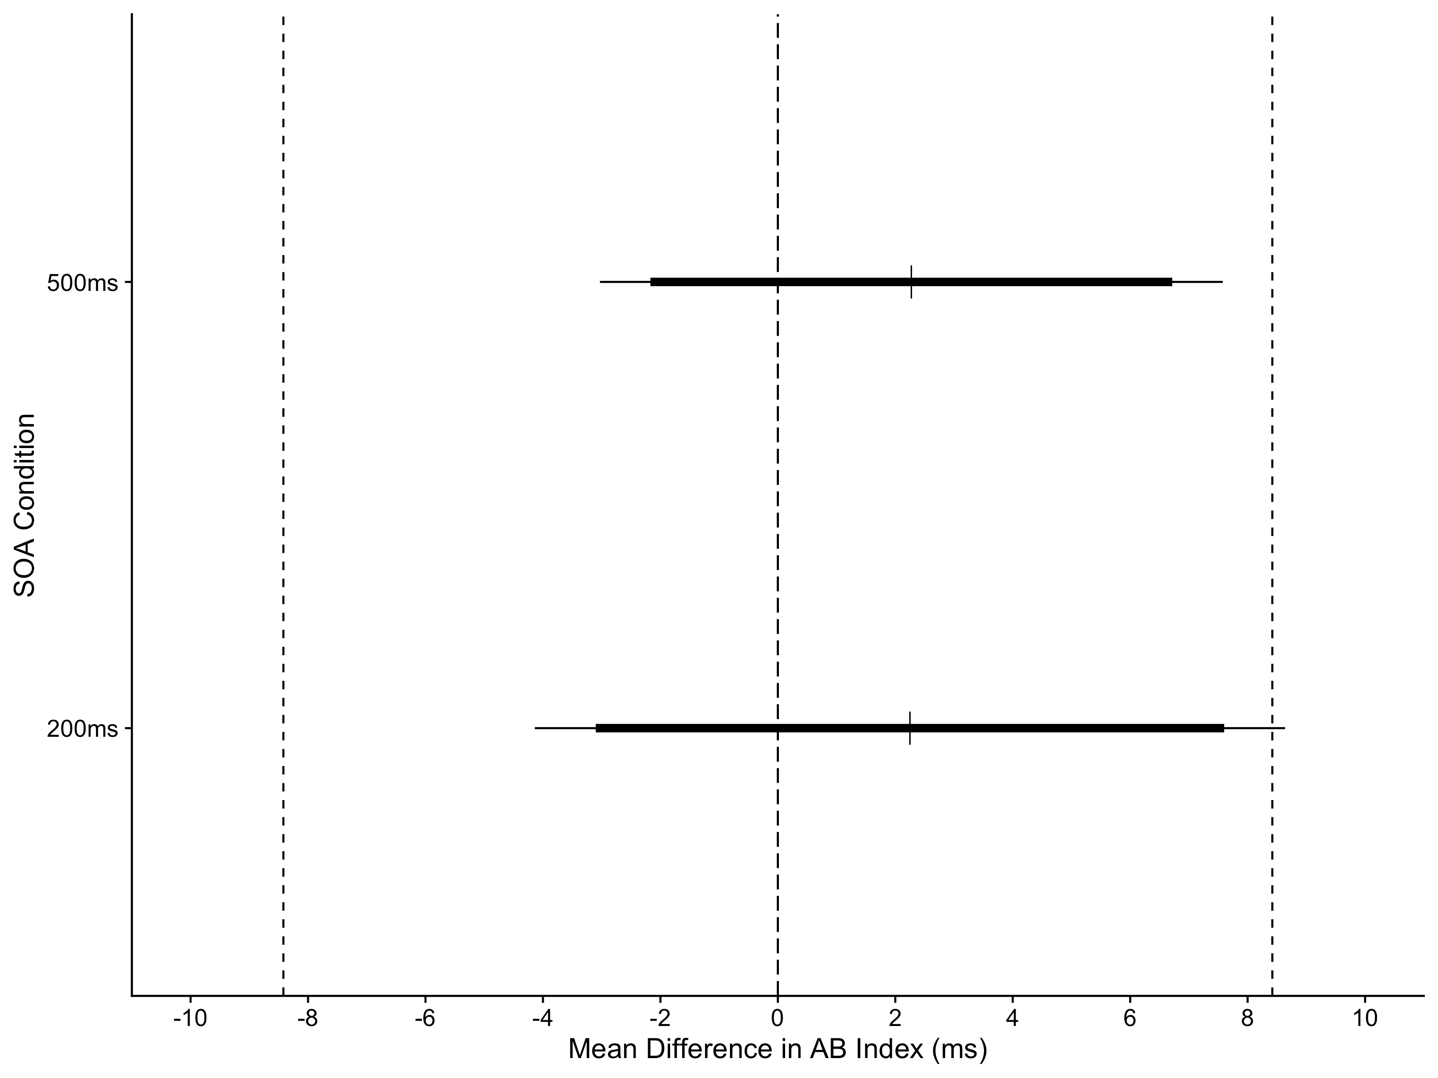
\includegraphics[width=\linewidth]{media/image1.jpeg}
    \caption{Diagram showing the trial procedure of the visual probe task. Each trial started with a fixation cross lasting 250ms. The fixation cross is then flanked by one of the stimulus pairs on the left and right. The stimuli remained on the screen for 200ms or 500ms depending on the SOA condition. The stimuli disappear and one image is replaced with a small dot. Participants had up to 2000ms to respond whether the dot was on the left or right. The next trial started with a new blank fixation cross.
    }

    \label{fig:1}
  \end{fullwidth}


\end{figure}

\begin{table}[h!]


  \begin{fullwidth}
    \caption{Mean (SD) values for participant characteristics and scale scores.}
    \label{tab:1}
    \begin{tabularx}{\linewidth}{@{}>{\RaggedRight\arraybackslash}X  l  l@{}}

      \toprule
                                           & {Non-Daily Smokers} & {Daily Smokers} \\ \midrule
      Age                                  & 28.68 (7.71)        & 31.84 (9.7)     \\
      \% female                            & 46.67{\%}           & 26.42{\%}       \\
      \% white                             & 93{\%}              & 92{\%}          \\
      FTCD                                 & 0.52 (1.31)         & 2.58 (2.17)     \\
      Cigarettes per day                   & 2.38 (2.74)         & 8.59 (6.41)     \\
      Age started to smoke                 & 18.51 (3.65)        & 17.93 (3.47)    \\
      Time since last cigarette (minutes)* & 2880 (4590)         & 60 (633.75)     \\ \bottomrule
    \end{tabularx}


    \small
    \emph{Note.} *Due to large skew, these values represent the median and IQR.
  \end{fullwidth}
\end{table}
Each trial started with a 250ms central fixation cross before two images were presented horizontally to the left and right. The content and duration of the two images was controlled by two variables: trial type and SOA. Trial type consisted of three conditions (neutral, smoking, or non-smoking) while SOA consisted of two conditions (200ms or 500ms). At picture offset, a small dot appeared in the location vacated by one of the images. The dot remained on the screen until the participant responded either left (Z key) or right (M key). After the participant responded the next trial began, with the screen containing only the fixation cross. The trial procedure is shown visually in Figure~\ref{fig:1}.

The trial type condition was based on 16 image pairs for neutral trials and 16 image pairs for smoking and non-smoking trials, meaning 32 unique image pairs in total. For neutral trials, the dot replaced either of the neutral image pairs. For smoking trials, the dot replaced a smoking image presented next to a matched non-smoking image. For non-smoking trials, the dot replaced a non-smoking image presented next to a smoking image.

We used 16 image pairs from the International Affective Picture System \parencite{Lang2008} for the neutral trials. We developed a series of matching smoking and non-smoking images for the smoking and non-smoking trials \parencite{Bartlett2020}. The list of IAPS images is available on the OSF project (\url{https://osf.io/fwud6/}), and our smoking/non-smoking images are available on the Gorilla open materials page.

The trial order was randomized with each picture pair presented four times to cover each combination of image (left and right) and dot location (left and right). This combination determined the trial type condition, where a left smoking image, right non-smoking image, and left dot would produce a smoking trial. For each picture pair, this process was repeated twice for each SOA condition, producing 384 trials split into two blocks with 64 trials in each SOA and trial type condition.
























\begin{figure}[t]

  \begin{fullwidth}
    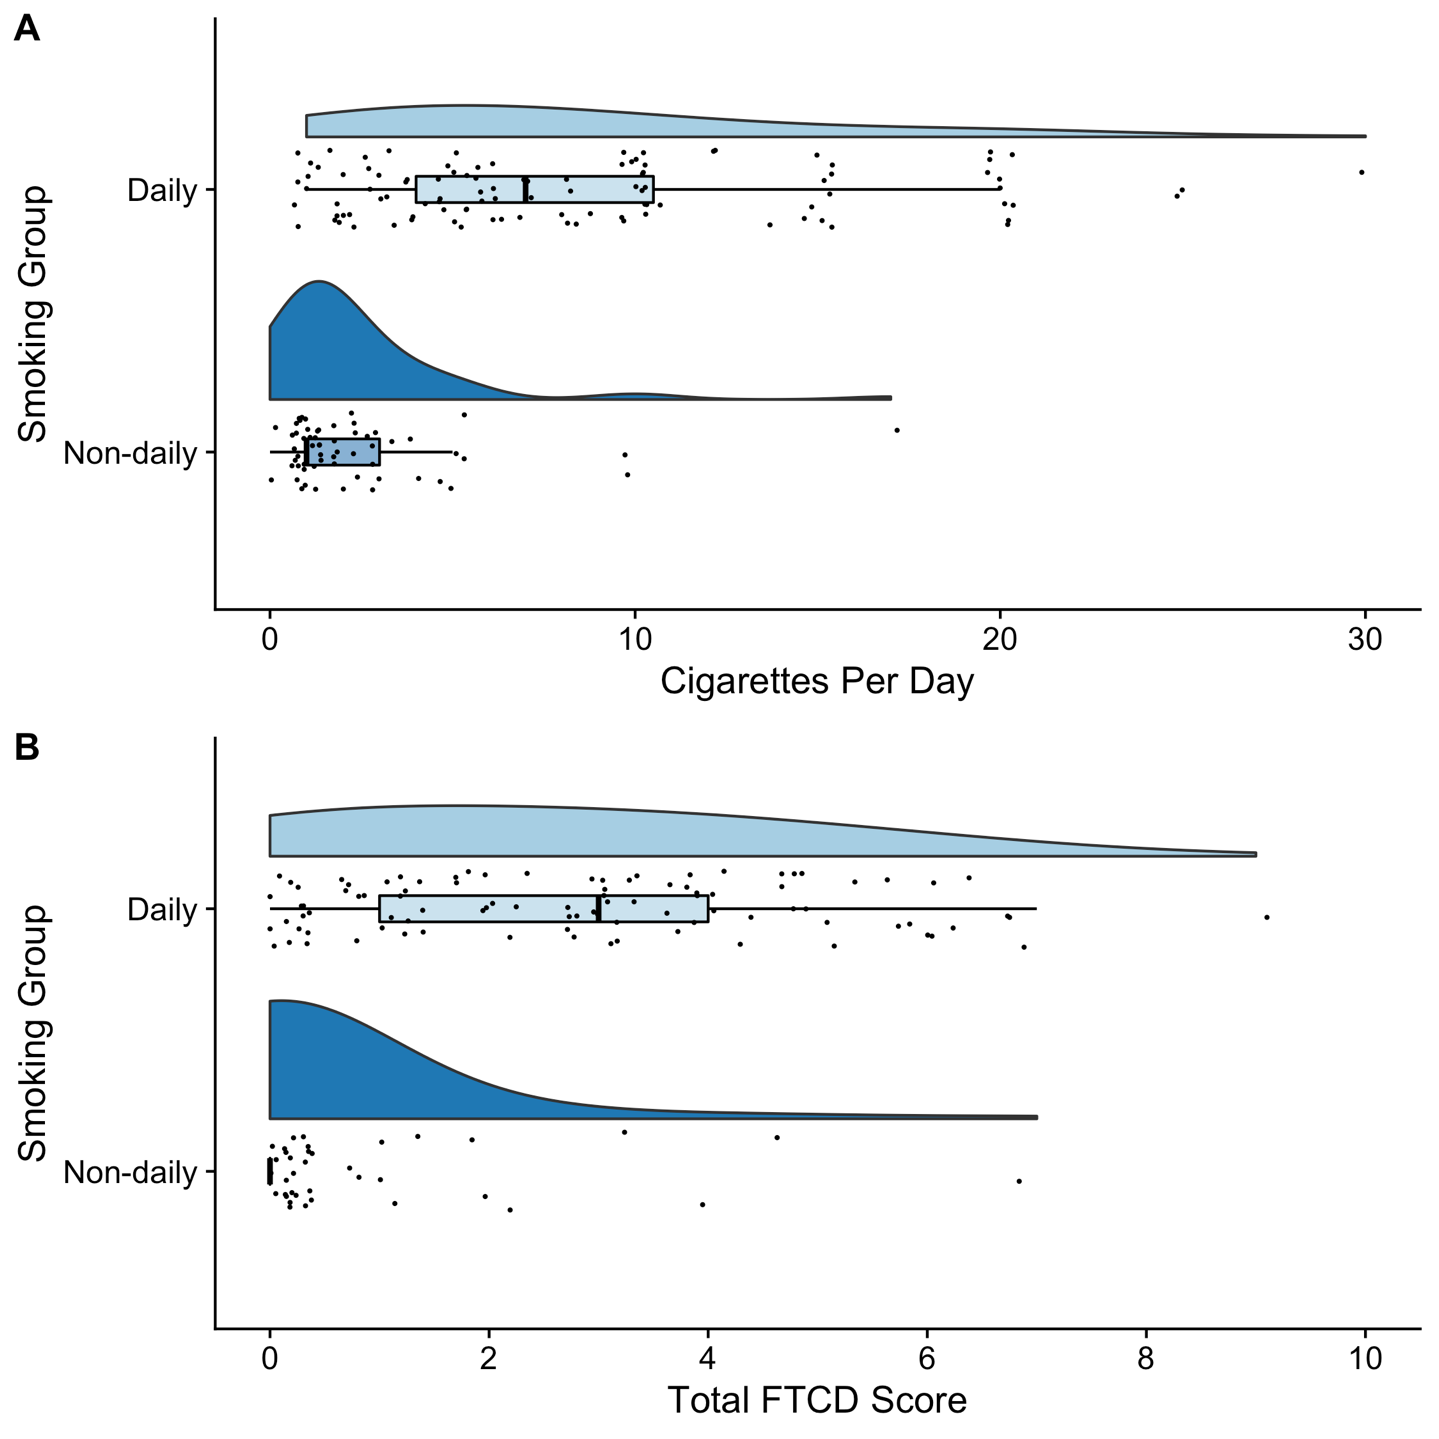
\includegraphics[width=\linewidth]{media/image2.jpeg}
    \caption{
      Two different measures of nicotine dependence: (A) number of cigarettes per day, and (B) FTCD score. The data are presented as raincloud plots \parencite{Allen2019}. The top element for each group represents the distribution of scores through the density. The bottom element presents the individual data points with a superimposed boxplot.
    }
    \label{fig:2}

  \end{fullwidth}

\end{figure}

\subsection{Procedure}

We provided participants with an information sheet, and they provided informed consent by ticking a box. This study was approved by the Ethical Approval board of the Faculty of Health and Life Sciences at Coventry University, United Kingdom (project reference number P88261). Participants completed a short questionnaire on their demographic information, smoking habits, and the FTCD. The next page contained the visual probe task which began with a set of instructions asking the participant to complete the task in a quiet environment free of distractions. Participants completed 12 practice trials which provided feedback on their responses and overall accuracy. After the task, participants reported whether they experienced any technical issues, whether they used an ineligible device, and if they had completed the study before. Like \textcite{Clifford2014}, we asked participants if they had any distractions while they completed the study such as listening to music. Finally, participants read a debriefing sheet before they were redirected to Prolific. If the participants successfully reached the end of the study, they were paid £2.

\section{Results}

\subsection{Participant Attrition and Demographics}

In total, 218 people accessed the study, 205 of whom completed the experiment and received payment. The final sample was 166 after applying exclusion criteria: 60 non-daily and 106 daily smokers. Participants were excluded for having fewer than 50\% of the possible trials (\emph{n} = 4), experiencing technical issues (\emph{n} = 16), reporting to smoke every day but not every week (\emph{n} = 3), and not smoking in the past four weeks (\emph{n} = 19). The total number of exclusions equals 42 as some participants met more than one criterion.

Table~\ref{tab:1} displays the demographic information of the selected participants. Daily smokers smoked more cigarettes per day and had a higher FTCD score than non-daily smokers. Non-daily smokers clearly displayed infrequent smoking behavior as the median time since their last cigarette was 48 hours compared to only 1 hour for daily smokers. Figure~\ref{fig:2} shows the distribution of FTCD scores and cigarettes per day.


































\subsection{Data Processing}

The R code for all analyses is available on the OSF (\url{https://osf.io/gm4jr/}). We removed incorrect responses in addition to responses faster than 200ms as they represent preemptive responses. We considered outliers to be any response outside 2.5 times the median absolute deviation for each participant, SOA, and trial condition \parencite{Leys2013}. This meant we removed 9.72\% of the total possible trials, with the median number of excluded trials for each participant being 23 (range 7 - 98).

For the confirmatory analyses, we focused on smoking/non-smoking image pairs and excluded the neutral pairs. Originally, we planned on conducting exploratory analyses to create orienting and disengagement indices \parencite{Salemink2007} by subtracting the mean RT to neutral trials from smoking trials (orienting) or non-smoking trials (disengagement), but a coding error meant we did not have matching numbers of neutral trials in the 200ms and 500ms SOA conditions. Therefore, we focused on our confirmatory analyses and excluded neutral trials.

\begin{figure}[t]

  \begin{fullwidth}
    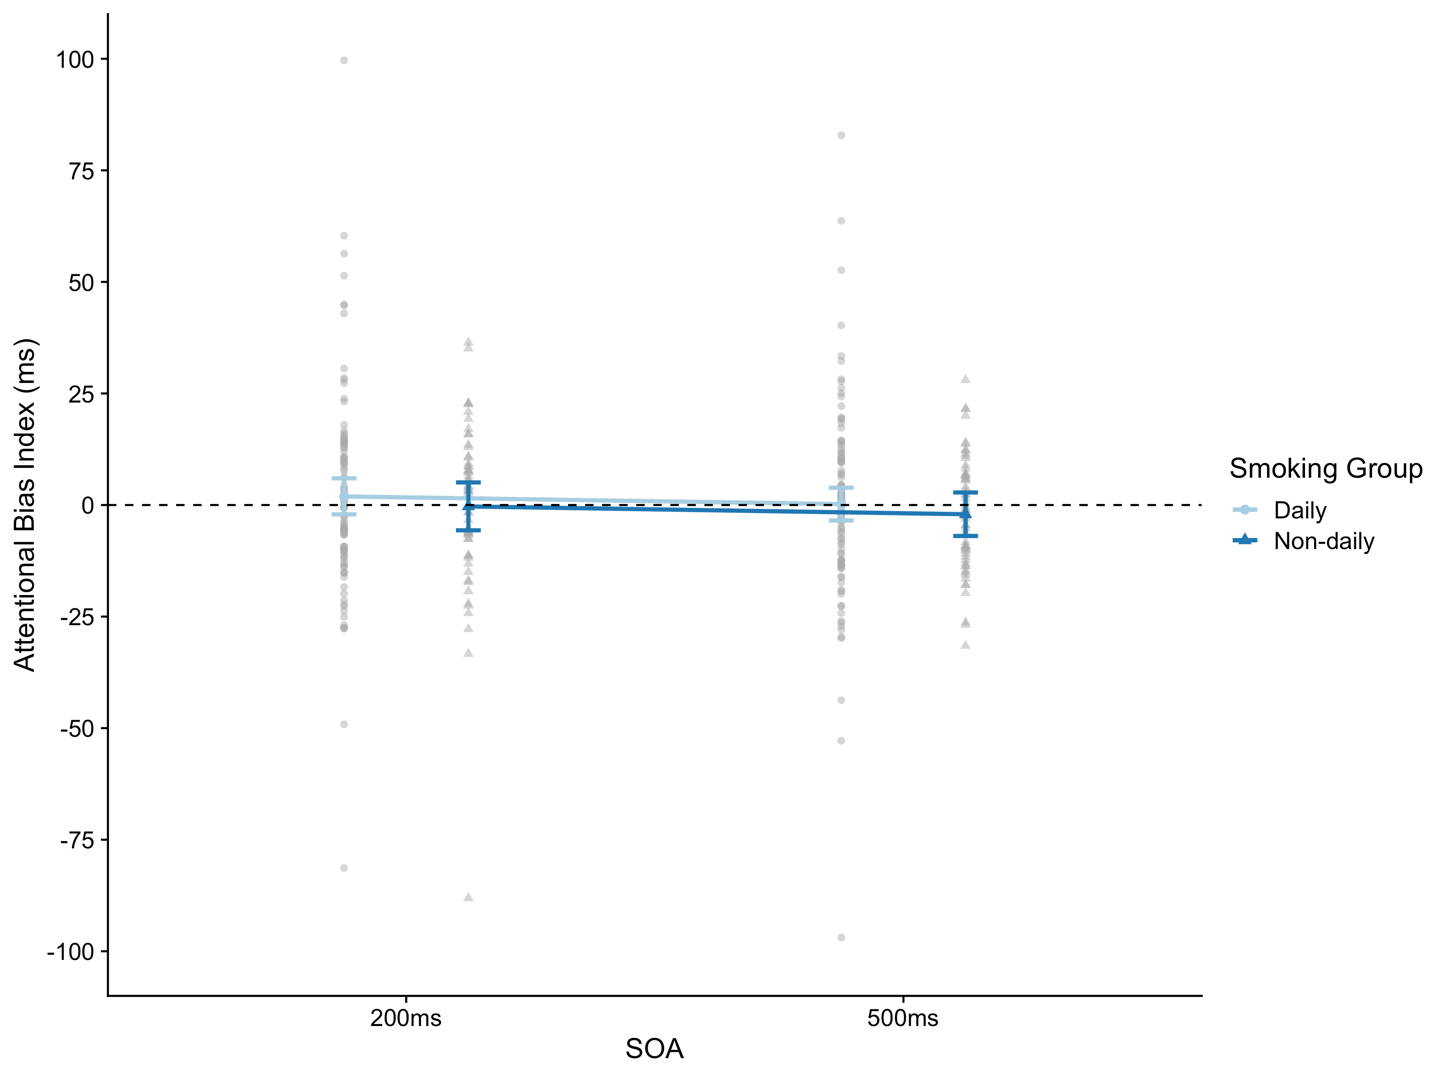
\includegraphics[width=\linewidth]{media/image3.jpeg}
    \caption{Interaction plot showing the mean attentional bias index for daily and non-daily smokers by SOA condition. The error bars represent the 95\% CI around the mean. Positive values indicate greater attentional bias towards smoking cues. The grey points show the individual scores per condition.}
    \label{fig:3}

  \end{fullwidth}


\end{figure}

After removing outliers, we calculated the mean RT to probes that replaced non-smoking images and the mean RT to probes that replaced smoking images. We then calculated the difference between these two values as our attentional bias index (non-smoking - smoking), where positive values mean faster average responses to smoking images. For each participant, this produced two values: one for the attentional bias index using a 200ms SOA and one for a 500ms SOA.
\subsection{Confirmatory Analyses: Attentional Bias Towards Smoking Cues}

The mean (\emph{SD}) attentional bias index in the 200ms SOA condition was 1.95ms (22.31) for daily smokers and -0.30ms (18.57) for non-daily smokers. In the 500ms SOA condition, the mean bias index was 0.21ms (21.93) for daily smokers and -2.06ms (12.67) for non-daily smokers. This was in the opposite direction to our hypothesis as we expected non-daily smokers to display greater attentional bias towards smoking images than daily smokers. The detailed results are displayed in Figure~\ref{fig:3}.

We used a 2 x 2 mixed ANOVA with SOA as a within-subjects IV and smoking group as a between-subjects IV. The mean attentional bias index was the DV. There was not a significant effect of SOA (\emph{F} (1, 164) = 0.58, \emph{p} (1, 164) = 0.58, \emph{p} = .448, $\hat{\eta}_{G}^{2}$ = .002) or smoking group (\emph{F} (1, 164) = 0.58,\emph{p} (1, 164) = 0.97, \emph{p} = .325, $\hat{\eta}_{G}^{2}$ = .003). There was also no significant interaction between the two factors, \emph{F} (1, 164) = 0.58, \emph{p} (1, 164) = 0.01, \emph{p} = .996, $\hat{\eta}_{G}^{2}$ < .001. These results do not support our prediction that non-daily smokers show greater attentional bias towards smoking images than daily smokers.


























\subsection{Exploratory Analyses: No Meaningful Difference in Attentional Bias}

To demonstrate there was no meaningful difference between daily and non-daily smokers, we performed equivalence testing on the two comparisons of interest: the difference between daily and non-daily smokers at each SOA condition. One cannot directly provide evidence in favor of the null hypothesis using traditional null hypothesis significance testing. Equivalence testing applies two one-sided tests to user-defined boundaries representing effects considered too small to be practically or theoretically meaningful \parencite{Lakens2018}. If both tests are statistically significant, one can conclude that the observed effect size is statistically equivalent to zero based on the boundaries.

There are different approaches to setting the boundaries for your smallest effect size of interest. We used Cohen's \emph{d} = ±0.41 based on the small telescopes method \parencite{Lakens2018}. The small telescopes method uses a sensitivity power analysis where you enter the sample size of a target study and calculate what effect size it would have 33\% power to detect. In our case, we used two groups of 25 and 26 participants based on \textcite{Vollstädt-Klein2011}, which would have 33\% power to detect an effect size of \emph{d} = ±0.41 (\emph{α} = .05). The small telescopes method is appropriate when previous research did not define their smallest effect size of interest, so it represents the effect size large enough to be detectable in the original study \parencite{Simonsohn2015}. Considering alternative choices for the effect size boundaries, our conclusions below hold when we use the larger effect size from our power analysis (10ms) but not when we use the smaller effect size (5ms). Because we are arguing differences in attentional bias in daily and non-daily smokers may be smaller than reported in previous research, we focus on the results using the small telescopes method.
\begin{figure}[t]


  \begin{fullwidth}

    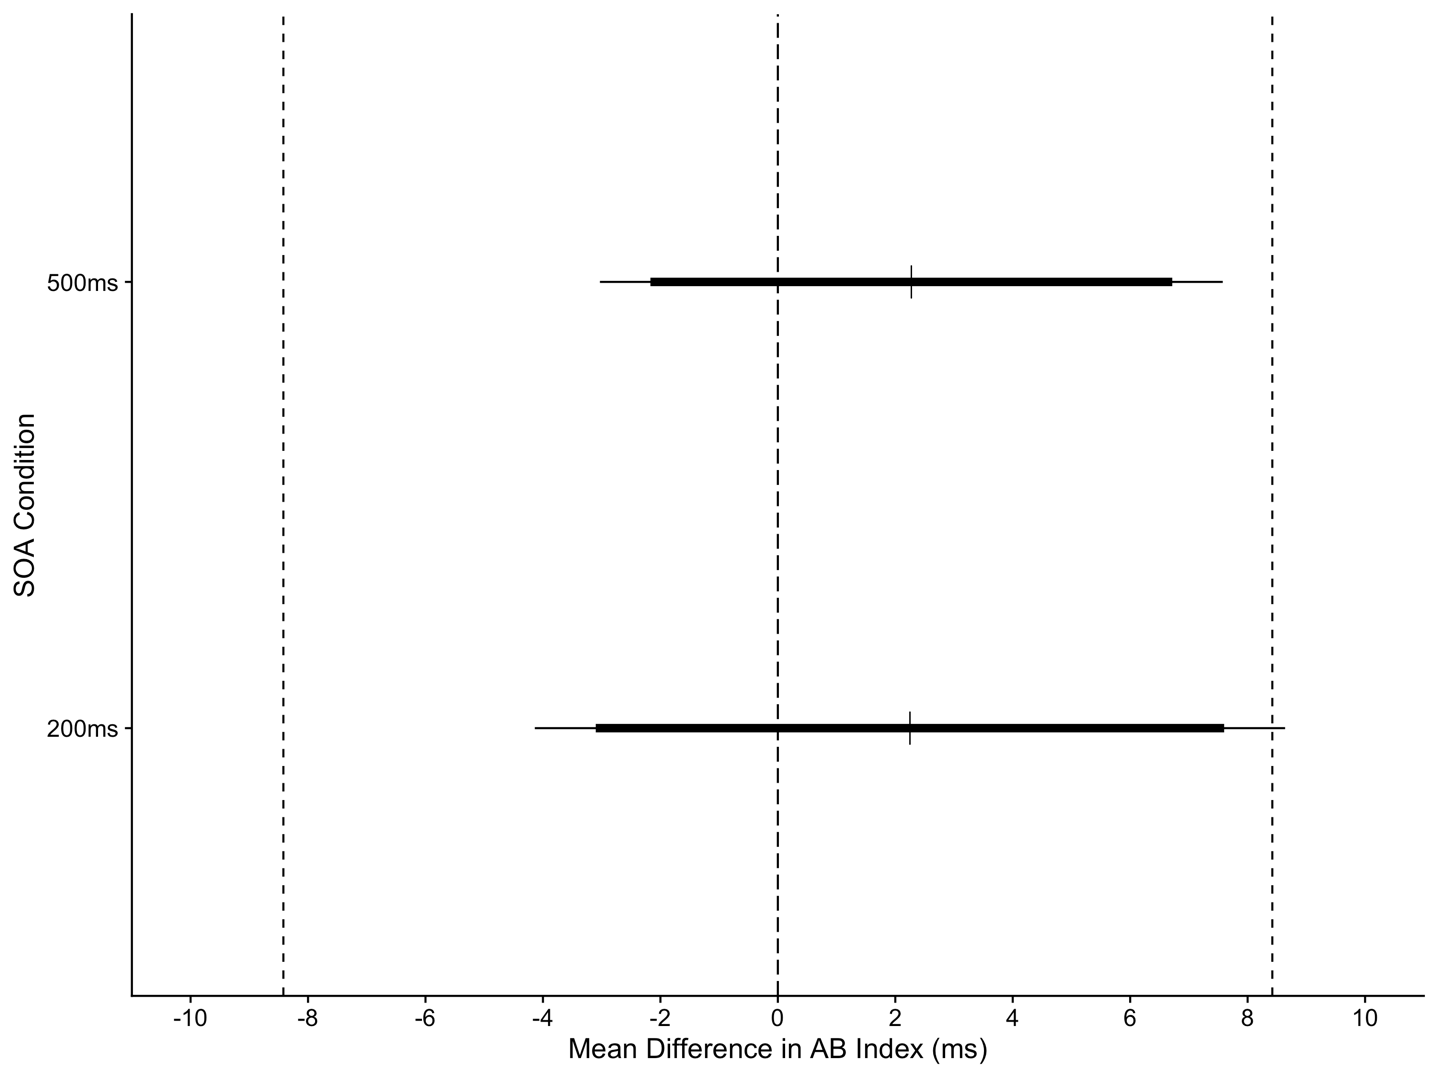
\includegraphics[width=\linewidth]{media/image4.jpeg}
    \caption{
      The thin vertical lines show the mean difference in attentional bias index between daily and non-daily smokers in each SOA condition. The thick horizontal black lines represent the 90\% CI for the two one-sided test procedure. The thin horizontal black lines represent the 95\% CI. The dashed vertical lines represent the equivalence boundaries in raw scores.}
    \label{fig:4}

  \end{fullwidth}


\end{figure}

For the 200ms SOA condition, the two one-sided test procedure was significant, demonstrating that the difference in attentional bias towards smoking images between daily and non-daily smokers was statistically equivalent to zero, \emph{t} (141.65) = -1.91, \emph{p} = .029. Similarly, the 500ms SOA condition was statistically equivalent to zero, \emph{t} (163.91) = -1.89, \emph{p}~=~.03. The equivalence testing procedure is presented in Figure~\ref{fig:4}, showing that the 90\% CI around the mean difference crosses zero, but does not cross the effect size boundaries of \emph{d}~=~±.41 (expressed here in raw units).






\subsection{Exploratory Analyses: Including trial type as an additional IV}

In our preregistration protocol, we focused on the attentional bias index as our outcome for confirmatory analyses, calculating it from the difference between smoking and neutral trials. While there were no meaningful differences between smoking groups, both peer-reviewers questioned whether participants first showed an attentional bias effect towards smoking images. Therefore, we performed exploratory analyses where we included trial type as an additional within-subjects IV instead of calculating the difference in RT between each condition.

We used a 2 x 2 x 2 mixed ANOVA using RT as our DV, trial type and SOA as within-subject IVs, and smoking group as a between-subjects IV. The only significant effect was SOA (\emph{F} (1, 164) = 13.03, \emph{p} < .001, $\hat{\eta}_{G}^{2}$ = .002), which in isolation is not theoretically meaningful to us. None of the other effects were statistically significant.

Although there were no significant effects including trial type, we quantified whether participants showed an attentional bias effect towards smoking images using the persons as effect sizes approach \parencite{Grice2020}. Instead of calculating a blanket mean difference between groups or conditions, one could quantify how many participants behaved consistent with theoretical predictions. In this context, we can ask how many participants showed faster RTs to smoking trials compared to non-smoking trials.

For each participant, we coded whether the difference in RT was negative (faster average responses to non-smoking images) or positive (faster average responses to smoking images), then calculated the percentage of participants showing a positive effect for each smoking group and SOA condition. Half (50\%) of daily smokers in the 200ms and 52.83\% in the 500ms SOA condition showed faster responses to smoking images. In contrast, 53.33\% of non-daily smokers in the 200ms SOA condition showed faster responses to smoking images, while 43.33\% responded faster to smoking images in the 500ms SOA condition, suggesting more participants responded faster to non-smoking images. We visualized these results in Figure~\ref{fig:5} where each line represents a participant and the color shows whether they responded faster to smoking or non-smoking images for each SOA condition and smoking group. Collectively, these exploratory analyses suggest participants did not display the predicted attentional bias effect towards smoking images.



























\begin{figure}[t]

  \begin{fullwidth}
    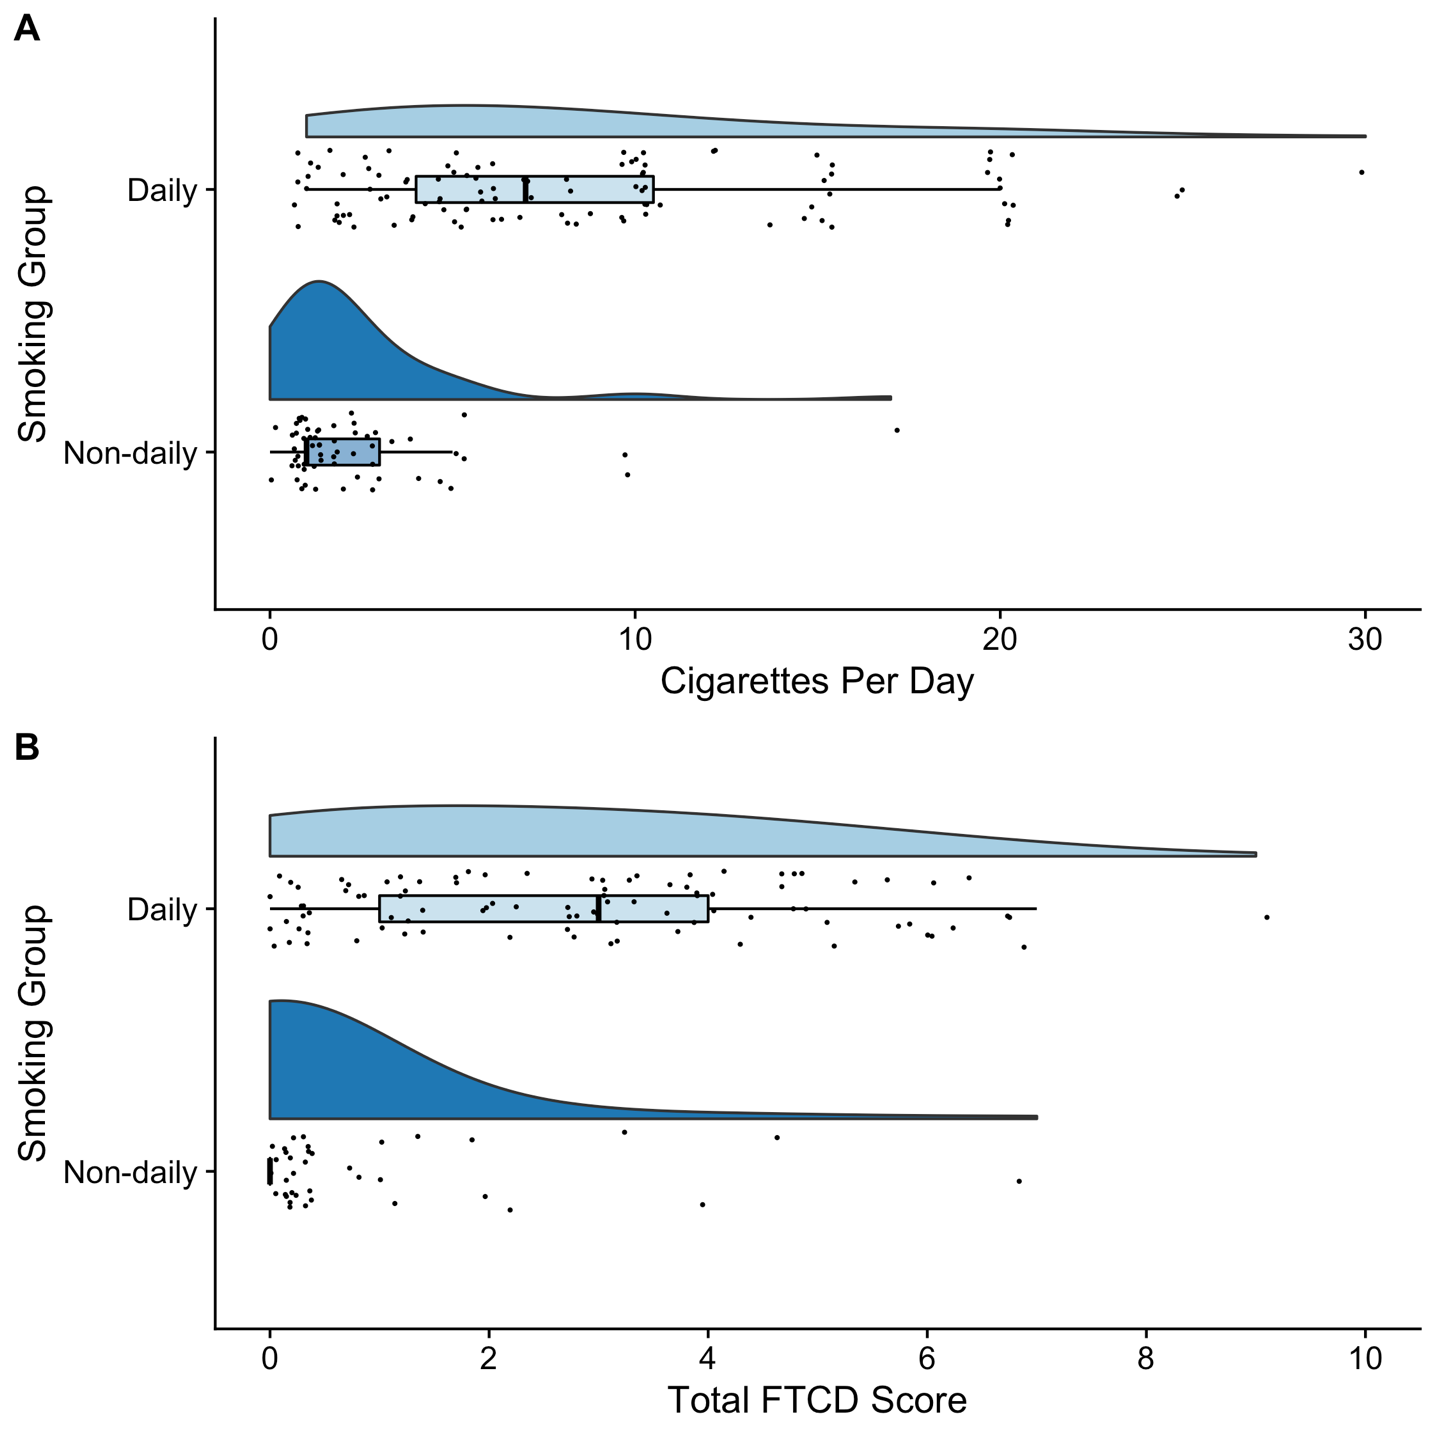
\includegraphics[width=\linewidth]{media/image5.jpeg}
    \caption{
      A dot plot visualizing whether each participant showed the predicted attentional bias effect towards smoking images. Each line represents one participant where their average RT to non-smoking and smoking images is connected. Positive slopes (purple lines) show participants who responded faster on average to non-smoking images while negative slopes (orange lines) show participants who responded faster on average to smoking images. Each panel represents the combination of smoking group and SOA condition.
    }
    \label{fig:5}
  \end{fullwidth}


\end{figure}


\subsection{Exploratory Analyses: Visual Probe Task Reliability}

Across the 16 smoking and non-smoking stimulus pairs, we calculated Cronbach's alpha for the attentional bias index which was poor for both the 200ms (\emph{α} = .29, 95\% \emph{CI} = [.00, .58]) and 500ms (\emph{α} = .19, 95\% \emph{CI} = [.00, .42]) SOA conditions.

We reported internal consistency estimates for comparison with previous studies, but these assume the items or trials are presented in the same order \parencite{Parsons2019}. As cognitive tasks randomize trials, internal consistency may not be the best approach. An alternative is a permutation approach to calculating split-half reliability \parencite{Parsons2020}. This randomly splits the data set into two halves many times and calculates the average correlation between each half. Using 5000 iterations, poor reliability was also reflected in the split-half estimate (corrected using the Spearman-Brown formula) for the 200ms (\emph{r} = .56, 95\% \emph{CI} = [.37, .7]) and 500ms (\emph{r} = .47, 95\% \emph{CI} = [.27, .62]) SOA conditions.

\section{Discussion}

We hypothesized that non-daily smokers would display greater attentional bias towards smoking cues than daily smokers. Existing literature showed ambiguous results. Some studies found that non-daily smokers exhibited greater attentional bias \parencite{Bradley2003, Hogarth2003, Mogg2005}, whereas others found that daily smokers displayed greater attentional bias \parencite{Chanon2010, Vollstädt-Klein2011, Zack2001}. Using traditional methods that calculate an attentional bias index from average differences in RT, the current study found no significant differences, with equivalence testing showing that there was no meaningful difference in attentional bias in daily and non-daily smokers.

We may have found null results as previous research could have problems with inflated effect sizes due to low statistical power. The previous largest sample was 51 smokers in \textcite{Vollstädt-Klein2011}. Splitting these into 25 and 26 participants, a sensitivity power analysis indicates that this sample size would be sensitive to detect effect sizes of Cohen's \emph{d} = 0.80 (\emph{α} = .05, power = .80). Incidentally, \textcite{Schaefer2019} showed that the median Cohen's \emph{d} in a random selection of 684 non-pre-registered articles was 0.80. In the long run, our study would have 99.80\% power to detect an effect size of \emph{d} = 0.80. Therefore, it is unlikely the effect size between daily and non-daily smokers is this large; if it was, we would have had enough power to detect it. Our study had the largest known sample size to investigate attentional bias with 60 non-daily smokers and 106 daily smokers. A sensitivity power analysis shows that this was sensitive to detect effect sizes of Cohen's \emph{d} = 0.46. Our study was sensitive to detect an effect size of almost half the size of \textcite{Vollstädt-Klein2011}. Yet our results were statistically equivalent to zero, meaning there may not be a meaningful difference in attentional bias between smoking groups, at least in its current implementation where the effect is assumed to represent stable trait-like group differences.

\begin{originalPurpose}

  Daily and non-daily smokers have different habits and motives but both groups find it difficult to quit smoking long-term. As attentional bias may be associated with addictive behavior, we used the visual probe task to compare daily and non-daily smokers. We predicted that non-daily smokers would show greater attentional bias towards smoking images than daily smokers. If non-daily smokers showed greater attentional bias, it would help to explain why they find it difficult to quit smoking while showing fewer signs of nicotine dependence.

\end{originalPurpose}

Contemporary theories suggest attentional bias may not be a trait-like phenomenon that can produce stable differences between groups. \textcite{Field2016} suggested that attentional bias varies depending on how substance cues are being evaluated. This theory suggests that rather than being a stable trait between groups, attentional bias fluctuates with the incentive value of a cue, making within-group differences more important. \textcite{Begh2016} found that laboratory measures like the visual probe task did not predict smoking behavior in the real-world. However, ecological momentary assessment of craving and awareness of smoking cues did predict smoking behavior. Therefore, the null results in our study may be a product of the fluctuating nature of attentional bias \parencite{Field2016}. In smaller samples, attentional bias could fluctuate one way or the other, but in larger samples (like our study) the differences could cancel out and converge to a mean difference around zero. Therefore, future research may benefit from investigating which factors affect the momentary evaluation of substance cues and the subsequent expression of attentional bias.



Using the visual probe task to measure factors that affect the momentary evaluation of substance cues may be problematic, though. There are vocal critics of the task due to its questionable level of internal consistency \parencite{Ataya2012, Schmukle2005, Waechter2014}. Our study also had suboptimal levels of internal consistency and split-half reliability. Researchers rarely report the reliability of cognitive tasks unless it is the focus of the article \parencite{Parsons2019}, which means it is difficult to assess how reliable the tasks were in previous smoking research. Experimental measures are designed to produce reliable differences between groups or condition, not consistently rank individuals \parencite{Hedge2018}. This means if researchers plan to use the visual probe task across multiple measurements - such as in cognitive bias modification or the evaluation of substance cues - its poor reliability is problematic. Future research should consider using eye-tracking as a direct measure of attentional bias as it produces larger effect sizes \parencite{Field2009}, has higher internal consistency \parencite{Price2015}, and higher criterion validity \parencite{Soleymani2020}.

\subsection{Limitations}

Our sample may have been more diverse in age and education than typical undergraduate samples, but it still contained predominantly white participants. Non-daily smoking is more prevalent in ethnic minority groups \parencite{Fagan2009, Levy2009} and the health implications of smoking disproportionately affect non-white smokers \parencite{StHelen2019}. Therefore, future research would benefit from recruiting a larger proportion of non-white smokers for the results to generalize beyond mostly white smokers.

The online nature of the study meant participants' smoking levels could not be verified objectively using measures like Carbon Monoxide \parencite{Wray2016}, but \textcite{Ramo2011} demonstrated that smoking-related information collected online has good reliability and validity. Relatedly, as participants completed the study online, there was no control over their smoking behavior before and during the study. This led to idiosyncrasies as some smokers reported smoking while they were completing the study. Although this may represent a more naturalistic environment for the smokers, our study had less control over smokers' deprivation levels.

\subsection{Conclusion}

The purpose of our study was to investigate the conflict in attentional bias results between daily and non-daily smokers. We expected non-daily smokers to show greater attentional bias towards smoking images than daily smokers. Greater attentional bias in non-daily smokers would have helped to explain why they find it difficult to quit smoking while showing fewer signs of nicotine dependence. However, there were no significant effects and using equivalence testing, we found that there was no meaningful difference in attentional bias between daily and non-daily smokers. The results can be interpreted in line with contemporary theories of attentional bias where there may not be stable trait-level differences between smoking groups in attentional bias. Future research should focus on investigating how attentional bias fluctuates over time using more reliable measures than the visual probe task.

\section{Disclosures}

\subsection{CRediT Contributions}

Conceptualization (JEB, RJ, NW); Methodology (JEB, RJ, NW); Formal analysis (JEB); Investigation (JEB); Data curation (JEB); Writing - original draft (JEB); Writing - Review \& editing (JEB); Supervision (RJ, NW).

\subsection{Data, code, and materials}

The data and code to reproduce these analyses are available on the OSF (\url{https://osf.io/am9hd/}). The OSF project contains all necessary files to reproduce the analyses and figures. The visual probe task was created in Gorilla and the task can be found using the open materials page (\url{https://gorilla.sc/openmaterials/85021})

\subsection{R Package Acknowledgements}

The results were created using R \parencite[version 4.1.3][]{RCoreTeam2020} and the R-packages \emph{afex} \parencite[version 1.0.1][]{Singmann2020}, \emph{cowplot} \parencite[version 1.1.1][]{Wilke2019}, \emph{dplyr} \parencite[version 1.0.10][]{Wickham2020}, \emph{ggplot2} \parencite[version 3.3.5][]{Wickham2016}, \emph{janitor} \parencite[version 2.1.0][]{Firke2019}, \emph{papaja} \parencite[version 0.1.1][]{Aust2022}, \emph{psych} \parencite[version 2.2.3][]{Revelle2019}, \emph{pwr} \parencite[version 1.3.0][]{Champely2020}, \emph{readr} \parencite[version 2.1.2][]{Wickham2018}, \emph{shiny} \parencite[version 1.7.1][]{Chang2020}, \emph{splithalf} \parencite[version 0.8.2][]{Parsons2020}, \emph{stringr} \parencite[version 1.4.0][]{Wickham2019}, \emph{tibble} \parencite[version 3.1.6][]{Müller2020}, \emph{tidyr} \parencite[version 1.2.0][]{Wickham2020}, \emph{tinylabels} \parencite[version 0.2.3][]{Barth2022}, and \emph{TOSTER} \parencite[version 0.4.0][]{Lakens2017}.

% \section{References}

% Allen, M., Poggiali, D., Whitaker, K., Marshall, T. R., \& Kievit, R. A. (2019). Raincloud plots: A multi-platform tool for robust data visualization. \emph{Wellcome Open Research}, \emph{4}, 63. https://doi.org/10.12688/wellcomeopenres.15191.1

% Anwyl-Irvine, A., Massonnié, J., Flitton, A., Kirkham, N., \& Evershed, J. (2019). Gorilla in our Midst: An online behavioral experiment builder. \emph{Behavior Research Methods}, \emph{52}, 388--407. https://doi.org/10.1101/438242

% Ataya, A. F., Adams, S., Mullings, E., Cooper, R. M., Attwood, A. S., \& Munafò, M. R. (2012). Internal reliability of measures of substance-related cognitive bias. \emph{Drug and Alcohol Dependence}, \emph{121}(1), 148--151. https://doi.org/10.1016/j.drugalcdep.2011.08.023

% Aust, F., \& Barth, M. (2020). \emph{papaja: Create APA manuscripts with R Markdown}. https://github.com/crsh/papaja

% Barth, M. (2022). \emph{tinylabels: Lightweight variable labels}. https://cran.r-project.org/package=tinylabels

% Bartlett, J. E. (2020). \emph{Daily and Non-daily Smokers: A Profile of Drive and Cognitive Control Mechanisms} [PhD thesis, Coventry University]. https://thesiscommons.org/h9gpe/

% Baschnagel, J. S. (2013). Using mobile eye-tracking to assess attention to smoking cues in a naturalized environment. \emph{Addictive Behaviors}, \emph{38}(12), 2837--2840. https://doi.org/10.1016/j.addbeh.2013.08.005

% Begh, R., Smith, M., Ferguson, S. G., Shiffman, S., Munafò, M. R., \& Aveyard, P. (2016). Association between smoking-related attentional bias and craving measured in the clinic and in the natural environment. \emph{Psychology of Addictive Behaviors}, \emph{30}(8), 868--875. https://doi.org/10.1037/adb0000231

% Bogdanovica, I., Godfrey, F., McNeill, A., \& Britton, J. (2011). Smoking prevalence in the European Union: A comparison of national and transnational prevalence survey methods and results. \emph{Tobacco Control}, \emph{20}(1), 1--9. https://doi.org/10.1136/tc.2010.036103

% Bradley, B. P., Mogg, K., Wright, T., \& Field, M. (2003). Attentional bias in drug dependence: Vigilance for cigarette-related cues in smokers. \emph{Psychology of Addictive Behaviors}, \emph{17}(1), 66--72. https://doi.org/10.1037/0893-164X.17.1.66

% Champely, S. (2020). \emph{Pwr: Basic functions for power analysis}. https://CRAN.R-project.org/package=pwr

% Chang, W., Cheng, J., Allaire, J., Xie, Y., \& McPherson, J. (2020). \emph{Shiny: Web application framework for r}. https://CRAN.R-project.org/package=shiny

% Chanon, V. W., Sours, C. R., \& Boettiger, C. A. (2010). Attentional bias toward cigarette cues in active smokers. \emph{Psychopharmacology}, \emph{212}(3), 309--320. https://doi.org/10.1007/s00213-010-1953-1

% Clifford, S., \& Jerit, J. (2014). Is There a Cost to Convenience? An Experimental Comparison of Data Quality in Laboratory and Online Studies. \emph{Journal of Experimental Political Science}, \emph{1}(2), 120--131. https://doi.org/10.1017/xps.2014.5

% Ehrman, R. N., Robbins, S. J., Bromwell, M. A., Lankford, M. E., Monterosso, J. R., \& O'Brien, C. P. (2002). Comparing attentional bias to smoking cues in current smokers, former smokers, and non-smokers using a dot-probe task. \emph{Drug and Alcohol Dependence}, \emph{67}(2), 185--191. https://doi.org/10.1016/S0376-8716(02)00065-0

% Fagan, P., \& Rigotti, N. A. (2009). Light and intermittent smoking: The road less traveled. \emph{Nicotine \& Tobacco Research}, \emph{11}(2), 107--110. https://doi.org/10.1093/ntr/ntn015

% Fagerström, K. (2012). Determinants of Tobacco Use and Renaming the FTND to the Fagerström Test for Cigarette Dependence. \emph{Nicotine \& Tobacco Research}, \emph{14}(1), 75--78. https://doi.org/10.1093/ntr/ntr137

% Field, M., \& Cox, W. M. (2008). Attentional bias in addictive behaviors: A review of its development, causes, and consequences. \emph{Drug and Alcohol Dependence}, \emph{97}(1-2), 1--20. https://doi.org/10.1016/j.drugalcdep.2008.03.030

% Field, M., Munafò, M. R., \& Franken, I. H. A. (2009). A meta-analytic investigation of the relationship between attentional bias and subjective craving in substance abuse. \emph{Psychological Bulletin}, \emph{135}(4), 589--607. https://doi.org/10.1037/a0015843

% Field, M., Werthmann, J., Franken, I., Hofmann, W., Hogarth, L., \& Roefs, A. (2016). The role of attentional bias in obesity and addiction. \emph{Health Psychology}, \emph{35}(8), 767--780. https://doi.org/10.1037/hea0000405

% Firke, S. (2019). \emph{Janitor: Simple tools for examining and cleaning dirty data}. https://CRAN.R-project.org/package=janitor

% Grice, J. W., Medellin, E., Jones, I., Horvath, S., McDaniel, H., O'lansen, C., \& Baker, M. (2020). Persons as Effect Sizes. \emph{Advances in Methods and Practices in Psychological Science}, \emph{3}(4), 443--455. https://doi.org/10.1177/2515245920922982

% Heatherton, T. F., Kozlowski, L. T., Frecker, R. C., \& Fagerström, K.-O. (1991). The Fagerström Test for Nicotine Dependence: A revision of the Fagerstrom Tolerance Questionnaire. \emph{British Journal of Addiction}, \emph{86}(9), 1119--1127. https://doi.org/10.1111/j.1360-0443.1991.tb01879.x

% Hedge, C., Powell, G., \& Sumner, P. (2018). The reliability paradox: Why robust cognitive tasks do not produce reliable individual differences. \emph{Behavior Research Methods}, \emph{50}(3), 1166--1186. https://doi.org/10.3758/s13428-017-0935-1

% Hogarth, L. C., Mogg, K., Bradley, B. P., Duka, T., \& Dickinson, A. (2003). Attentional orienting towards smoking-related stimuli: \emph{Behavioural Pharmacology}, \emph{14}(2), 153--160. https://doi.org/10.1097/00008877-200303000-00007

% Kang, O.-S., Chang, D.-S., Jahng, G.-H., Kim, S.-Y., Kim, H., Kim, J.-W., Chung, S.-Y., Yang, S.-I., Park, H.-J., Lee, H., \& Chae, Y. (2012). Individual differences in smoking-related cue reactivity in smokers: An eye-tracking and fMRI study. \emph{Progress in Neuro-Psychopharmacology and Biological Psychiatry}, \emph{38}(2), 285--293. https://doi.org/10.1016/j.pnpbp.2012.04.013

% Kotz, D., Fidler, J., \& West, R. (2012). Very low rate and light smokers: Smoking patterns and cessation-related behaviour in England, 2006-11: Very low rate and light smokers. \emph{Addiction}, \emph{107}(5), 995--1002. https://doi.org/10.1111/j.1360-0443.2011.03739.x

% Lakens, D. (2017). Equivalence tests: A practical primer for t-tests, correlations, and meta-analyses. \emph{Social Psychological and Personality Science}, \emph{1}, 1--8. https://doi.org/10.1177/1948550617697177

% Lakens, D., Scheel, A. M., \& Isager, P. M. (2018). Equivalence Testing for Psychological Research: A Tutorial. \emph{Advances in Methods and Practices in Psychological Science}, \emph{1}(2), 259--269. https://doi.org/10.1177/2515245918770963

% Lang, P. J., Bradley, M. M., \& Cuthbert, B. N. (2008). \emph{International affective picture system (IAPS): Affective ratings of pictures and instruction manual. Technical Report A-8. Gainesville: University of Florida}.

% Levy, D. E., Biener, L., \& Rigotti, N. A. (2009). The natural history of light smokers: A population-based cohort study. \emph{Nicotine \& Tobacco Research}, \emph{11}(2), 156--163. https://doi.org/10.1093/ntr/ntp011

% Leys, C., Ley, C., Klein, O., Bernard, P., \& Licata, L. (2013). Detecting outliers: Do not use standard deviation around the mean, use absolute deviation around the median. \emph{Journal of Experimental Social Psychology}, \emph{49}(4), 764--766. https://doi.org/10.1016/j.jesp.2013.03.013

% Mogg, K., Bradley, B. P., Field, M., \& De Houwer, J. (2003). Eye movements to smoking-related pictures in smokers: Relationship between attentional biases and implicit and explicit measures of stimulus valence. \emph{Addiction}, \emph{98}(6), 825--836. https://doi.org/10.1046/j.1360-0443.2003.00392.x

% Mogg, K., Field, M., \& Bradley, B. P. (2005). Attentional and approach biases for smoking cues in smokers: An investigation of competing theoretical views of addiction. \emph{Psychopharmacology}, \emph{180}(2), 333--341. https://doi.org/10.1007/s00213-005-2158-x

% Müller, K., \& Wickham, H. (2020). \emph{Tibble: Simple data frames}. https://CRAN.R-project.org/package=tibble

% Parsons, S. (2020). \emph{Splithalf; robust estimates of split half reliability}. https://doi.org/10.6084/m9.figshare.5559175.v5

% Parsons, S., Kruijt, A.-W., \& Fox, E. (2019). Psychological Science Needs a Standard Practice of Reporting the Reliability of Cognitive-Behavioral Measurements. \emph{Advances in Methods and Practices in Psychological Science}, \emph{2}(4), 378--395. https://doi.org/10.1177/2515245919879695

% Pennington, C. R., Jones, A., Bartlett, J. E., Copeland, A., \& Shaw, D. J. (2021). Raising the bar: Improving methodological rigour in cognitive alcohol research. \emph{Addiction}, \emph{116}(11), 3243--3251. https://doi.org/https://doi.org/10.1111/add.15563

% Price, R. B., Kuckertz, J. M., Siegle, G. J., Ladouceur, C. D., Silk, J. S., Ryan, N. D., Dahl, R. E., \& Amir, N. (2015). Empirical Recommendations for Improving the Stability of the Dot-Probe Task in Clinical Research. \emph{Psychological Assessment}, \emph{27}(2), 365--376. https://doi.org/10.1037/pas0000036

% R Core Team. (2020). \emph{R: A language and environment for statistical computing}. R Foundation for Statistical Computing. https://www.R-project.org/

% Ramo, D. E., Hall, S. M., \& Prochaska, J. J. (2011). Reliability and validity of self-reported smoking in an anonymous online survey with young adults. \emph{Health Psychology}, \emph{30}(6), 693--701. https://doi.org/10.1037/a0023443

% Revelle, W. (2019). \emph{Psych: Procedures for psychological, psychometric, and personality research}. Northwestern University. https://CRAN.R-project.org/package=psych

% Salemink, E., Hout, M. A. van den, \& Kindt, M. (2007). Selective attention and threat: Quick orienting versus slow disengagement and two versions of the dot probe task. \emph{Behaviour Research and Therapy}, \emph{45}(3), 607--615. https://doi.org/10.1016/j.brat.2006.04.004

% Schäfer, T., \& Schwarz, M. A. (2019). The Meaningfulness of Effect Sizes in Psychological Research: Differences Between Sub-Disciplines and the Impact of Potential Biases. \emph{Frontiers in Psychology}, \emph{10}, 1--13. https://doi.org/10.3389/fpsyg.2019.00813

% Schmukle, S. C. (2005). Unreliability of the dot probe task. \emph{European Journal of Personality}, \emph{19}(7), 595--605. https://doi.org/10.1002/per.554

% Shiffman, S. (2009). Light and intermittent smokers: Background and perspective. \emph{Nicotine \& Tobacco Research}, \emph{11}(2), 122--125. https://doi.org/10.1093/ntr/ntn020

% Shiffman, S., Dunbar, M. S., Li, X., Scholl, S. M., Tindle, H. A., Anderson, S. J., \& Ferguson, S. G. (2014). Smoking Patterns and Stimulus Control in Intermittent and Daily Smokers. \emph{PLoS ONE}, \emph{9}(3), 1--14. https://doi.org/10.1371/journal.pone.0089911

% Shiffman, S., Dunbar, M. S., Scholl, S. M., \& Tindle, H. A. (2012a). Smoking motives of daily and non-daily smokers: A profile analysis. \emph{Drug and Alcohol Dependence}, \emph{126}(3), 362--368. https://doi.org/10.1016/j.drugalcdep.2012.05.037

% Shiffman, S., Tindle, H., Li, X., Scholl, S., Dunbar, M., \& Mitchell-Miland, C. (2012b). Characteristics and smoking patterns of intermittent smokers. \emph{Experimental and Clinical Psychopharmacology}, \emph{20}(4), 264--277. https://doi.org/10.1037/a0027546

% Simonsohn, U. (2015). Small Telescopes: Detectability and the Evaluation of Replication Results. \emph{Psychological Science}, \emph{26}(5), 559--569. https://doi.org/10.1177/0956797614567341

% Singmann, H., Bolker, B., Westfall, J., Aust, F., \& Ben-Shachar, M. S. (2020). \emph{Afex: Analysis of factorial experiments}. https://CRAN.R-project.org/package=afex

% Soleymani, A., Ivanov, Y., Mathot, S., \& Jong, P. J. de. (2020). Free-viewing multi-stimulus eye tracking task to index attention bias for alcohol versus soda cues: Satisfactory reliability and criterion validity. \emph{Addictive Behaviors}, \emph{100}, 106117. https://doi.org/10.1016/j.addbeh.2019.106117

% St.Helen, G., Benowitz, N. L., Ahluwalia, J. S., Tyndale, R. F., Addo, N., Gregorich, S. E., Pérez-Stable, E. J., \& Cox, L. S. (2019). Black Light Smokers: How Nicotine Intake and Carcinogen Exposure Differ Across Various Biobehavioral Factors. \emph{Journal of the National Medical Association}, \emph{111}(5), 509--520. https://doi.org/10.1016/j.jnma.2019.04.004

% Tindle, H. A., \& Shiffman, S. (2011). Smoking Cessation Behavior Among Intermittent Smokers Versus Daily Smokers. \emph{American Journal of Public Health}, \emph{101}(7), e1--e3. https://doi.org/10.2105/AJPH.2011.300186

% Tong, E. K., Ong, M. K., Vittinghoff, E., \& Pérez-Stable, E. J. (2006). Nondaily Smokers Should Be Asked and Advised to Quit. \emph{American Journal of Preventive Medicine}, \emph{30}(1), 23--30. https://doi.org/10.1016/j.amepre.2005.08.048

% Vollstädt-Klein, S., Loeber, S., Winter, S., Leménager, T., Goltz, C. von der, Dinter, C., Koopmann, A., Wied, C., Winterer, G., \& Kiefer, F. (2011). Attention Shift towards Smoking Cues Relates to Severity of Dependence, Smoking Behavior and Breath Carbon Monoxide. \emph{European Addiction Research}, \emph{17}(4), 217--224. https://doi.org/10.1159/000327775

% Waechter, S., Nelson, A. L., Wright, C., Hyatt, A., \& Oakman, J. (2014). Measuring Attentional Bias to Threat: Reliability of Dot Probe and Eye Movement Indices. \emph{Cognitive Therapy and Research}, \emph{38}(3), 313--333. https://doi.org/10.1007/s10608-013-9588-2

% Wickham, H. (2016). \emph{ggplot2: Elegant graphics for data analysis}. Springer-Verlag New York. https://ggplot2.tidyverse.org

% Wickham, H. (2019). \emph{Stringr: Simple, consistent wrappers for common string operations}. https://CRAN.R-project.org/package=stringr

% Wickham, H., \& Henry, L. (2020). \emph{Tidyr: Tidy messy data}. https://CRAN.R-project.org/package=tidyr

% Wickham, H., François, R., Henry, L., \& Müller, K. (2020). \emph{Dplyr: A grammar of data manipulation}. https://CRAN.R-project.org/package=dplyr

% Wickham, H., Hester, J., \& Francois, R. (2018). \emph{Readr: Read rectangular text data}. https://CRAN.R-project.org/package=readr

% Wilke, C. O. (2019). \emph{Cowplot: Streamlined plot theme and plot annotations for 'ggplot2'}. https://CRAN.R-project.org/package=cowplot

% Wray, J. M., Gass, J. C., Miller, E. I., Wilkins, D. G., Rollins, D. E., \& Tiffany, S. T. (2016). A Comparative Evaluation of Self-Report and Biological Measures of Cigarette Use in Non-Daily Smokers. \emph{Psychological Assessment}, \emph{28}(9), 1043--1050. https://doi.org/10.1037/pas0000227

% Zack, M., Belsito, L., Scher, R., Eissenberg, T., \& Corrigall, W. A. (2001). Effects of abstinence and smoking on information processing in adolescent smokers. \emph{Psychopharmacology}, \emph{153}(2), 249--257. https://doi.org/10.1007/s002130000552

\nocite{*}
\RaggedRight\printbibliography


\end{document}